\documentclass[a4paper]{article}
\usepackage{tikz}
\usepackage{amsmath} % Para \sqrt si lo deseas en alguna fórmula
\usepackage[margin=2cm]{geometry}

\begin{document}

\begin{center}
    \textbf{Distancia de un punto a una recta (euclidiana vs. manhattan)}
\end{center}

\begin{center}
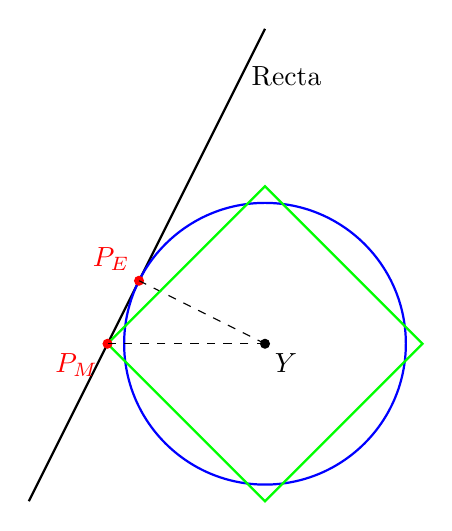
\begin{tikzpicture}[scale=2.0]
    % -----------------------------------------------------
    % 1) Definimos la recta: y = 2x + 2
    %    Trazada desde x = -2 (y=-2) hasta x = 1 (y=4)
    % -----------------------------------------------------
    \draw[thick] (-1.5,-1) -- (0,2) node[pos=0.9, right] {Recta};

    % -----------------------------------------------------
    % 2) Punto Y en el origen (0,0)
    % -----------------------------------------------------
    \filldraw (0,0) circle (0.8pt) node[below right] {$Y$};

    % -----------------------------------------------------
    % 3) Distancia Euclidiana: Círculo con centro en Y
    %    Radio = distancia perpendicular de Y a la recta = 2 / sqrt(5)
    %    Punto de tangencia Euclidiano (P_E) calculado = (-0.8, 0.4)
    % -----------------------------------------------------
    \draw[blue, thick] (0,0) circle ({2/sqrt(5)});
    % Punto de tangencia Euclidiano
    \filldraw[red] (-0.8, 0.4) circle (0.8pt) node[above left] {$P_E$};
    \draw[dashed] (0,0) -- (-0.8, 0.4);

    % -----------------------------------------------------
    % 4) Distancia Manhattan: Rombo (L1) con "radio" = 1
    %    El rombo (o diamante) de L1 = 1 tiene vértices (1,0), (0,1), (-1,0), (0,-1)
    %    Punto de tangencia Manhattan (P_M) = (-1,0)
    % -----------------------------------------------------
    % Dibujamos el rombo
    \draw[green, thick]
        (0,1) -- (1,0) -- (0,-1) -- (-1,0) -- cycle;
    % Punto de tangencia Manhattan
    \filldraw[red] (-1,0) circle (0.8pt) node[below left] {$P_M$};
    \draw[dashed] (0,0) -- (-1,0);

\end{tikzpicture}
\end{center}

\end{document}
